\newcommand{\prevalence}{
    \begin{tikzpicture}
        \begin{axis}[
            height=5.5cm,
            width=9cm,
            xmin=2019,
            xmax=2051,,
            ymin=0,
            axis lines=left,
            xlabel={Year},
            ylabel={Estimated number of\\dementia patients},
            ylabel style={align=center, font=\normalfont\linespread{0.9}\selectfont},,
            xtick={2020, 2030, 2040, 2050},
            xticklabels={2020, 2030, 2040, 2050}
        ]
            \addplot[
                red,
                thick,
                mark=*
            ] coordinates {
                (2019, 57.4)
                (2030, 83.2)
                (2040, 116)
                (2050, 152.8)
            };
            \addplot [name path=lower, draw=none] coordinates {
                (2019, 50.4)
                (2030, 73)
                (2040, 100.7)
                (2050, 130.8)
            };
            \addplot [name path=upper, draw=none] coordinates {
                (2019, 65.1)
                (2030, 94.6)
                (2040, 132.1)
                (2050, 175.9)
            };
            \addplot [
                fill=red!20,
                draw=none
            ] fill between[of=upper and lower];
        \end{axis}
    \end{tikzpicture}
}

\newcommand{\stickman}[2]{
    \node[circle,fill,minimum size=2.5mm,#2] (head) at #1 {};
    \node[rounded corners=1pt,minimum height=0.65cm,minimum width=0.2cm,fill,below = 0.5pt of head,#2] (body) {};
    \draw[line width=0.5mm,round cap-round cap,#2] ([shift={(1pt,-0.5pt)}]body.north east) --++(-90:3mm);
    \draw[line width=0.5mm,round cap-round cap,#2] ([shift={(-1pt,-0.5pt)}]body.north west)--++(-90:3mm);
    \draw[thick,white,-round cap] (body.south) --++(90:2.75mm);
}

\newcommand{\heterogeneity}[1]{
    \begin{tikzpicture}
        \node[] at (-4, -3) {};
        \node[] at (4, 3) {};

        \stickman{(-3, -1.5)}{controls-default}
        \stickman{(-2.5, -1.4)}{controls-default}
        \stickman{(-3.1, -0.3)}{controls-default}
        \stickman{(-2.55, -0.25)}{controls-default}
        \stickman{(-2, -0.7)}{controls-default}
        \stickman{(-1.5, -1.1)}{controls-default}
        \stickman{(-2.8, 0.8)}{controls-default}
        \stickman{(-2.1, 0.5)}{controls-default}
        \stickman{(-1.5, 0.1)}{controls-default}
        \stickman{(-0.95, -1.45)}{controls-default}
        \stickman{(-0.95, 0.3)}{controls-default}
        \stickman{(-0.3, -0.7)}{controls-default}
        \stickman{(-2.95, 2)}{controls-default}
        \stickman{(-2.4, 1.8)}{controls-default}
        \stickman{(-1.9, 2.7)}{controls-default}
        \stickman{(-1.75, 1.5)}{controls-default}
        \stickman{(-1.2, 1.65)}{controls-default}
        \stickman{(-0.45, 0.7)}{controls-default}
        \stickman{(0.1, 0)}{controls-default}
        \stickman{(0.2, -1.1)}{controls-default}
        \stickman{(0.3, 1.2)}{controls-default}
        \stickman{(-0.3, 2.1)}{controls-default}
        \stickman{(0.6, 0.2)}{controls-default}
        \stickman{(0.7, -1.35)}{controls-default}

        \draw[densely dotted, thick, red] plot [smooth] coordinates {(0.3, 3) (0.8, 0.5) (1.5, -1.6) (2.1, -2.5)};
        \node[font=\footnotesize, text=red, anchor=north west] at (0.3, 3.2) {
            \textbf{Dementia patients}
        };

        \ifnum#1=0
            \stickman{(1.1, 1.05)}{cases-default}
            \stickman{(0.85, 2.4)}{cases-default}
            \stickman{(1.5, -0.2)}{cases-default}
            \stickman{(1.5, 2)}{cases-default}
            \stickman{(1.8, 0.95)}{cases-default}
            \stickman{(2.2, 2.1)}{cases-default}
            \stickman{(2.15, -1.1)}{cases-default}
            \stickman{(2.8, -1.45)}{cases-default}
            \stickman{(2.55, 0.6)}{cases-default}
            \stickman{(3.15, 1.1)}{cases-default}
            \stickman{(2.9, 2.45)}{cases-default}
        \fi
        \ifnum#1=1
            \stickman{(1.1, 1.05)}{cases-default!70!controls-default}
            \stickman{(0.85, 2.4)}{cases-default!40!controls-default}
            \stickman{(1.5, -0.2)}{cases-default!65!yellow}
            \stickman{(1.5, 2)}{cases-default}
            \stickman{(1.8, 0.95)}{cases-default!80!controls-default!50!yellow}
            \stickman{(2.2, 2.1)}{cases-default!55!controls-default!90!yellow}
            \stickman{(2.15, -1.1)}{cases-default!70!yellow!80!controls-default}
            \stickman{(2.8, -1.45)}{cases-default!30!yellow}
            \stickman{(2.55, 0.6)}{cases-default!45!controls-default!80!yellow}
            \stickman{(3.15, 1.1)}{cases-default!50!yellow}
            \stickman{(2.9, 2.45)}{cases-default}
        \fi
    \end{tikzpicture}
}
\begin{frame}{Dementia}
    \begin{tikzpicture}
        \node[] at (-5.25, -3.5) {};
        \node[] at (5.25, 3.5) {};

        \only<1>{
            \node[inner sep=0pt, draw=black] at (0, 0) {
                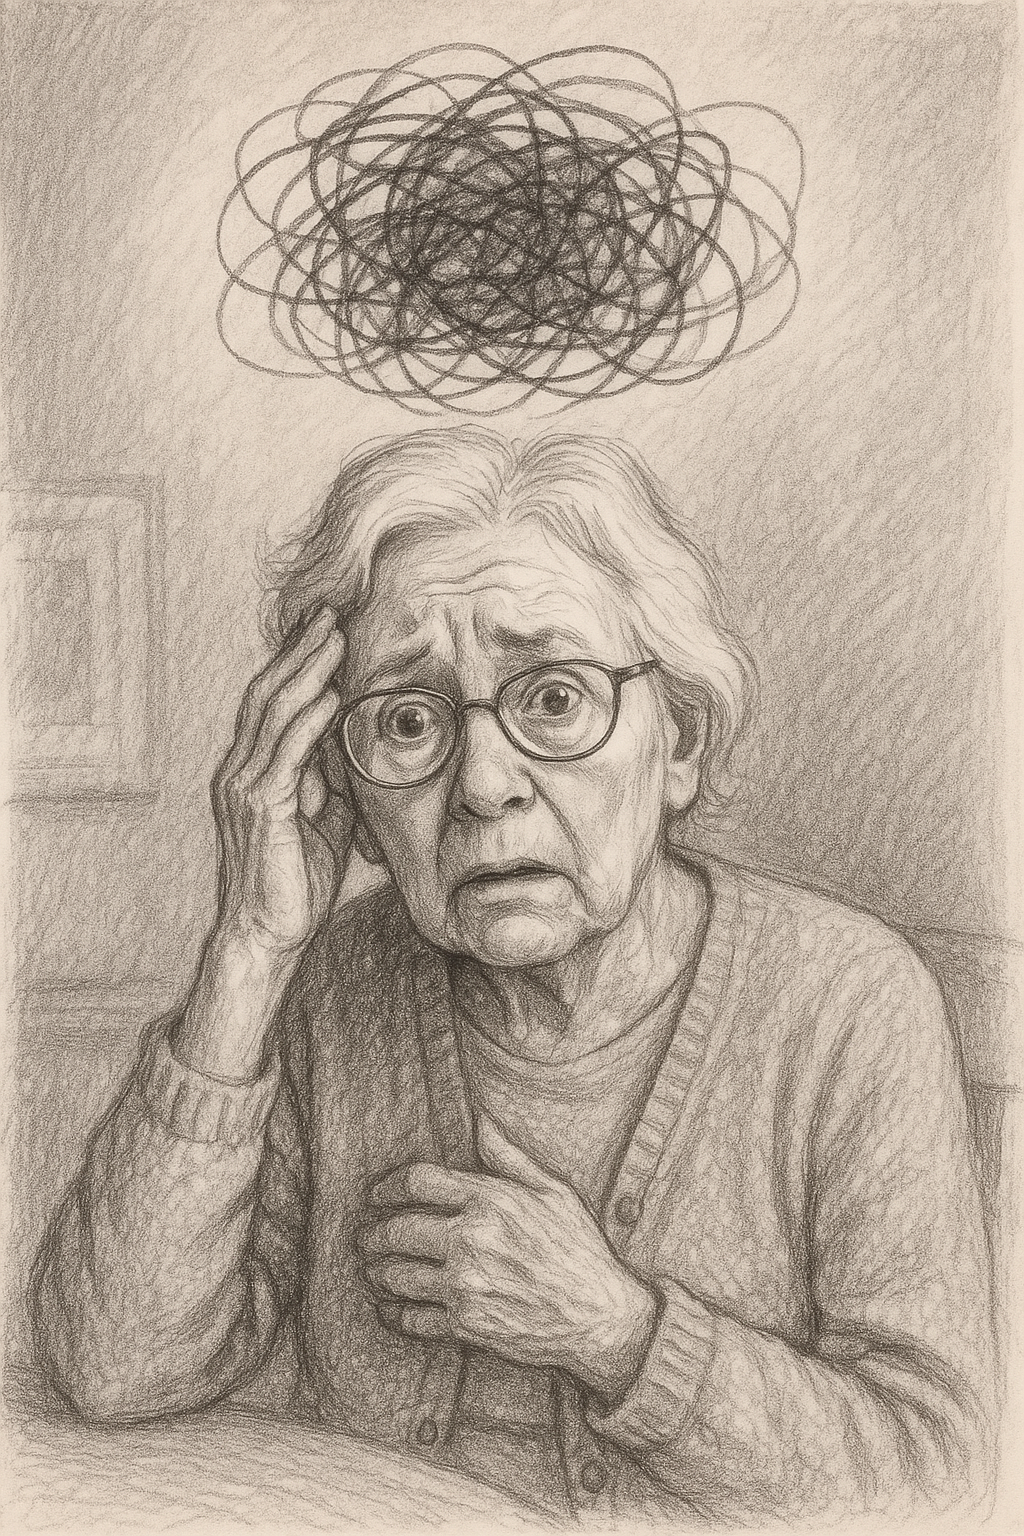
\includegraphics[width=4cm]{data/dementia_patient.png}
            };
            \node[anchor=south, font=\tiny, inner sep=0pt] at (0, -3.65) {
                Image generated by GPT-4o
            };
        }
        \only<2>{
            \mriside{-3}{0}{3cm}{1.5}{data/healthy_brain.png}
            \node[] at (-3, -2.65) {
                Healthy control
            };
            \mriside{3}{0}{3cm}{1.5}{data/ad_brain.png}
            \node[] at (3, -2.65) {
                Dementia patient
            };
            \node[anchor=south, font=\tiny, inner sep=0pt] at (0, -3.65) {
                Data from the Alzheimers Disease Neuroimaging Initiative (ADNI)
            };
        }
        \only<3>{
            \node[] at (0, 0.5) {
                \prevalence
            };
            \node[anchor=south, font=\tiny, inner sep=0pt, text width=10cm, align=flush center] at (0, -3.65) {
                Adapted from Nichols, E., et al. (2022). Estimation of the global prevalence of dementia in 2019 and forecasted prevalence in 2050: an analysis for the Global Burden of Disease Study 2019. The Lancet Public Health, 7(2), e105-e125.
            };
        }
        \only<4>{
            \node[] at (0, 0) {
                \heterogeneity{0}
            };
        }
        \only<5>{
            \node[] at (0, 0) {
                \heterogeneity{1}
            };
        }
        \only<6>{
            \node[] at (0, 0) {
                
\includegraphics[width=7cm]{data/ema.png}
            };
        }
    \end{tikzpicture}
\end{frame}
